\chapter{Literature Review} 
\label{chap:litrev}

This chapter presents the analysis and review of relevant literature conducted throughout this project. The research comprises of literature surrounding current solutions and risk-based route planning.

\section{Background}
\label{litrev:background}
This project is high in complexity. It utilises custom, user and system inputs into a data-driven route planning algorithm, displaying the output on an OpenStreetMap-based web application. 

This review begins with researching literature on existing systems and how they cater to a user's requirements. A review of competing products allowed for gaps in the current market to be identified, therefore developing an idea of requirements for the proposed system \see{litrev:competingproducts}. 

Furthermore, understanding how cyclists consider different risk factors when planning a ride was key in understanding what routing algorithm was implemented to fit the project's requirements best. An in-depth review of existing literature was conducted to understand two primary risk factors for cyclists: cycling infrastructure \see{litrev:cyclinginfrastructure} and weather conditions \see{litrev:weatherconditions}. 

\section{Research Methods}
\label{litrev:researchmethod}

An initial exploration of sources and subject areas was conducted using Google Chrome to comprehensively understand the topic at hand. Certain regions of interest were also highlighted through crowdsourcing ideas from knowledgeable individuals. After these areas were outlined, in-depth research was conducted primarily through Google Scholar and the EBSCO database. The Zotero plugin and app managed citations and bibliography items (\cite{noauthor_zotero_nodate}). All bibliography items have also been stored in a CSV file, utilising Zotero's export functionality; doing so ensures that all sources can be re-visited and are not lost after this project's conclusion.

\section{Competing Products}
\label{litrev:competingproducts}

There are many route planners available with many features, some common between applications and others specific to one. Applications like Plotaroute.com (\cite{noauthor_free_nodate}), Komoot (\cite{noauthor_komoot_nodate}) and Google Maps (\cite{noauthor_google_nodate}) have some commonalities, however, serve slightly different purposes \see{fig:solutionsandfeatures}\see{fig:research-results}.

\begin{figure}[h!]
    \centering
    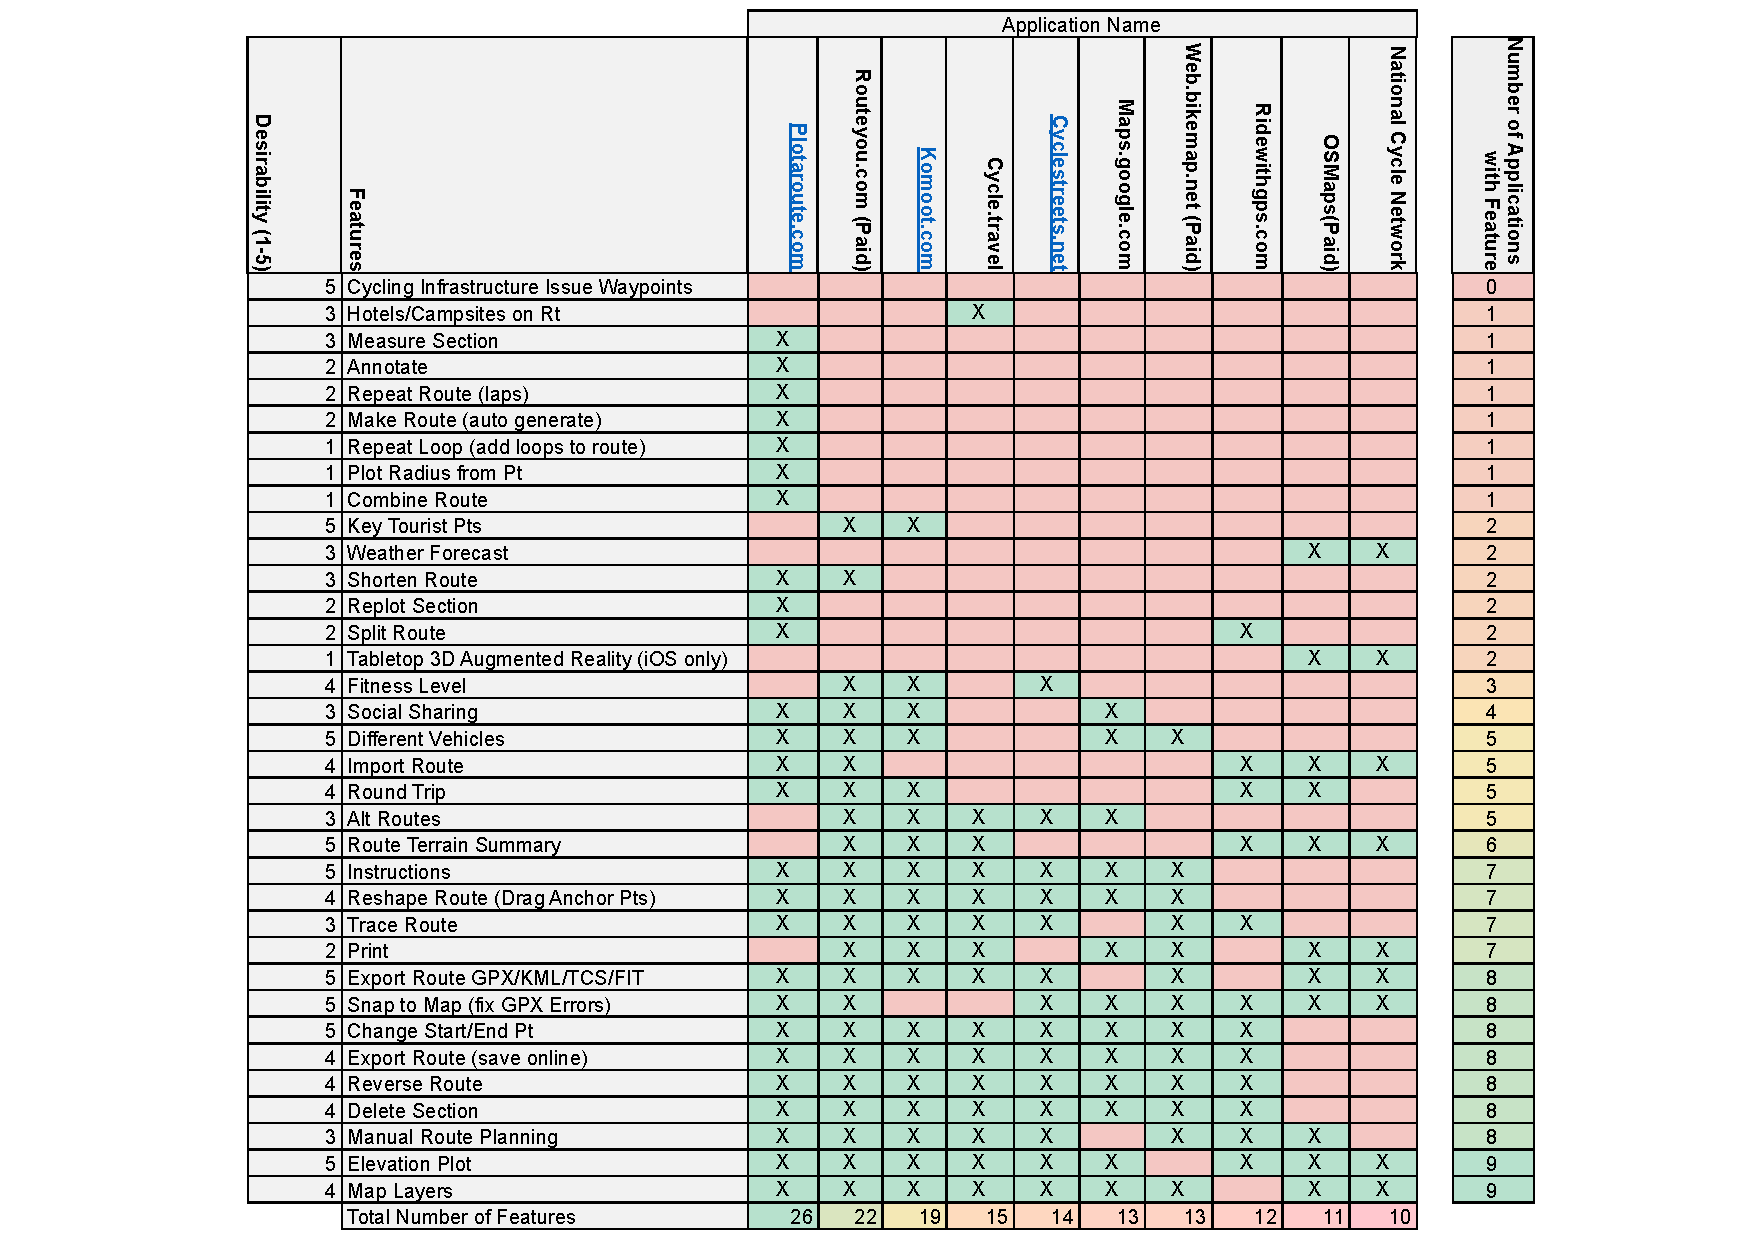
\includegraphics[width=1\linewidth]{figures/current_apps.pdf}
    \caption{Table of current solutions and their included features}
    \label{fig:solutionsandfeatures}
\end{figure}

\subsection{Plotaroute.com}
\label{litrev:plotaroute}
Plotaroute.com (\cite{noauthor_free_nodate}) (Plotaroute), contains a wide range of features, including nearly all features highlighted in Figure 2.1 \see{fig:solutionsandfeatures}. The User Interface (UI) was identified as the primary shortfall of Plotaroute. Its UI is cluttered due to the large number of features present in the application \see{fig:plotarouteui}. For first-time users, it can be initially confusing what each part of the application does. Due to this, it's unclear what type of route planner Plotaroute is, which will fundamentally affect a user's initial decision on whether to use the application.

\subsection{Komoot}
\label{litrev:komoot}
Komoot (\cite{noauthor_komoot_nodate}) offers a simpler-looking, feature-rich application for planning and discovering routes \see{fig:komootui}. The application has a community focus, where users can also discover or share routes. Consequently, this results in the user needing minimal effort when planning shorter, location-specific rides, however Komoot doesn't offer discovery of longer routes. When compared to Plotaroute, Komoot is more user-friendly without sacrificing core features. One primary setback with Komoot is that some route planning functionality is part of a paid-for service, therefore locking certain users out of some desirable functionality.

\subsection{Google Maps}
\label{litrev:gmaps}

Google Maps (\cite{noauthor_google_nodate}) trades the custom cycling functionality for a simple, multi-functional route planning application \see{fig:gmapsui}. Google Maps is likely the most user-friendly out of all the applications, simply due to its consistency across other Google applications (\cite{noauthor_material_nodate}). This has trade-offs, however, most cycling-specific functionality is not present, therefore the routing algorithm is restricted to its default configuration with little customisability.

\label{fig:research-results}
\begin{figure}[h!]
    \centering
    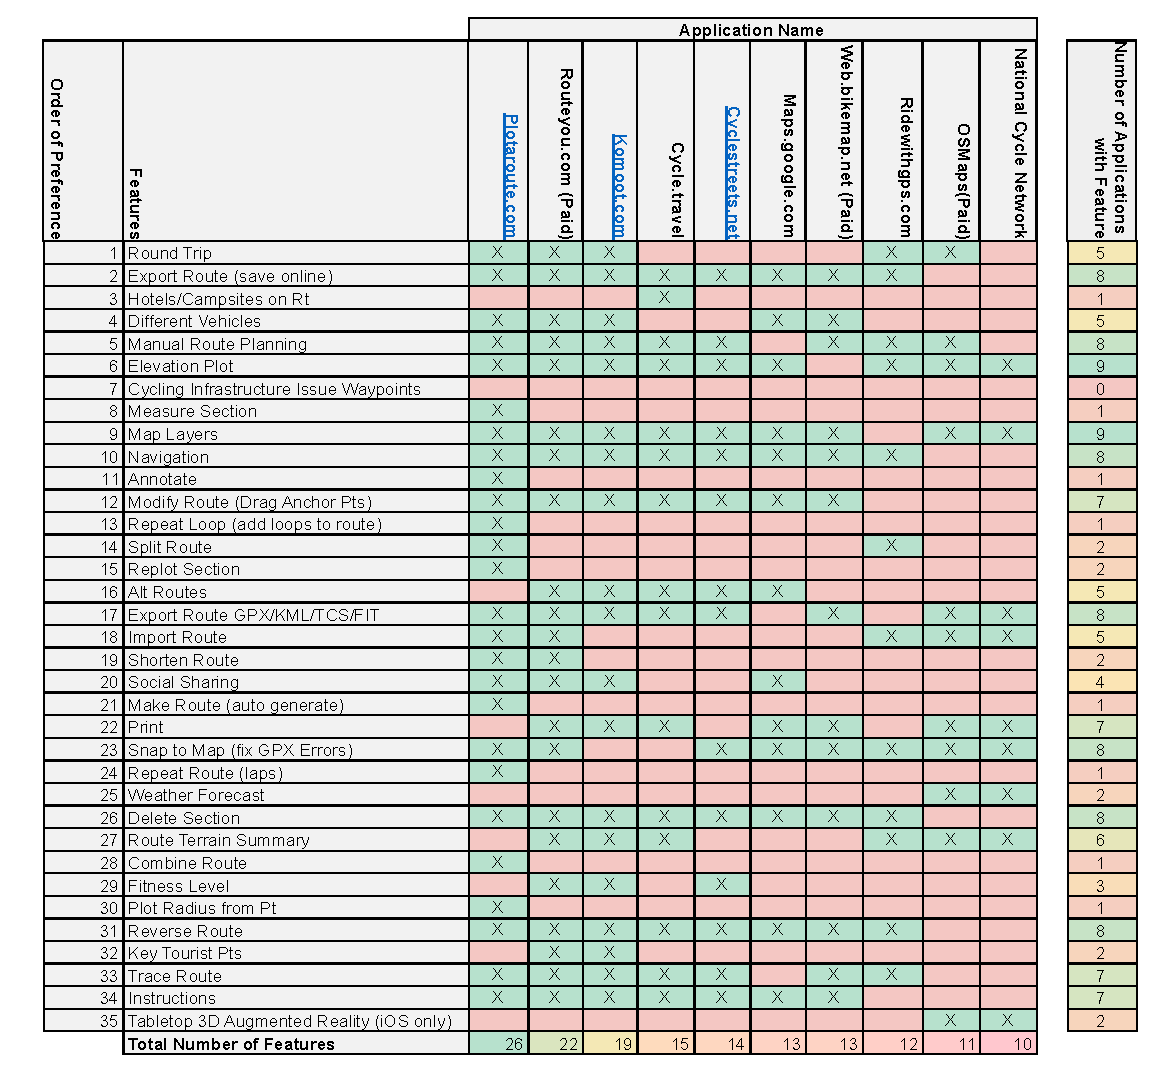
\includegraphics[width=1\linewidth]{figures/current_apps_post_research.pdf}
    \caption{Features in priority order based on user feedback}
    \label{fig:features}
\end{figure}

\section{Risk Factors in Route Planning}
Risk-based cycling route planning requires extensive knowledge of the impact of cycling and transportation infrastructure currently in place. It is also critical to understand how other external factors impact the risk of a route on an ever-changing basis. Within this section, a range of risk factors were explored to understand how multiple risk factors can be implemented into route planning algorithms.

\subsection{Cycling Infrastructure}
\label{litrev:cyclinginfrastructure}
The cycling infrastructure along a route must be understood because it is common for cyclists to share the same infrastructure as motorised vehicles. However, a cyclist has no physical protection if a crash occurs (\cite{reynolds_impact_2009}). There is often purpose-built infrastructure for cyclists, whether bike lanes alongside shared roads or off-road bike paths and this segregated infrastructure can help improve the safety of a route for a cyclist. Furthermore, Hong states how investing in effective cycling infrastructure "mitigates the negative effects of poor weather conditions" (\cite{hong_can_2020}), which further demonstrates that good, known infrastructure is key to improving the physical and perceived safety of a route in a range of different weather conditions. 

Furthermore, crowd-sourced data from route planners, cyclists and fitness applications such as Strava Routes (\cite{noauthor_strava_nodate}) have been key in developing new infrastructure. Boettge states how the most accurate assessment of a cycle network would come directly from the cyclists who use the network (\cite{boettge_assessing_2017}). Cyclists who use the network are the most familiar with the quality of each route and how traffic conditions improve the safety of the route. Utilising the GPS information from route planners and fitness tracking applications alongside direct input from cyclists can help build new routes and improve pre-existing routes, therefore preventing injuries and high-risk situations by modifying transportation infrastructure (\cite{reynolds_impact_2009}).

Areas with little to no cycling infrastructure, such as busy roads and roundabouts, force cyclists to have a heightened attentiveness that other road users don't have to consider due to not only the physical danger but the cyclists' perceived danger (\cite{doorley_analysis_2015}). These risks should be considered within route planning to decrease the number of 'risk' areas along a cyclist's route whilst also giving local areas the incentive to make infrastructure modifications to decrease the number of 'high-risk' points. Therefore, in the long-term, it will mitigate the need for constant action by cyclists to ensure their safety, which will, in turn, influence individuals' decisions to cycle (\cite{reynolds_impact_2009}).

Hull and O'Holleran also demonstrate how cities with a high reputation among cyclists also have safer roads and more attractive infrastructure. The Netherlands scored relatively equally amongst all categories, in comparison to cities with less of a reputation and, therefore, a lower standard of cycling infrastructure \see{fig:bicycleinfrastructurescorestable} \see{fig:bicycleinfrastructurescores} (\cite{hull_bicycle_2014}). This supports how Reynolds et al. further illustrate how investing in cycling infrastructure will greatly incentivise individuals to cycle due to the decreased risk. 

\begin{figure}
    \centering
    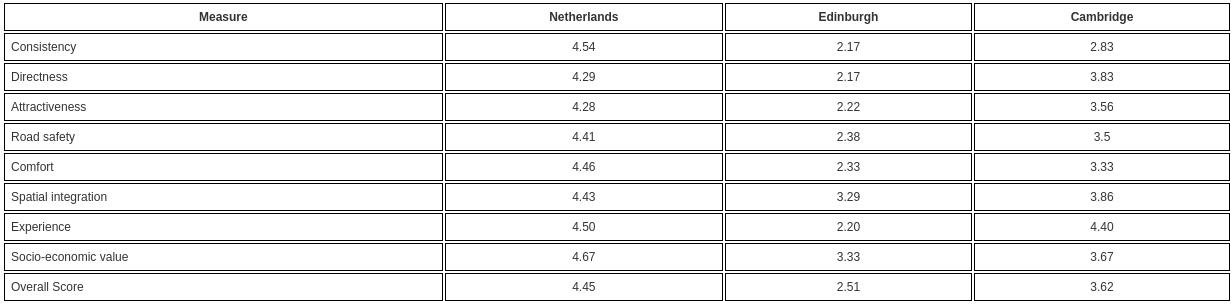
\includegraphics[width=400px, keepaspectratio]{figures/bicycle_infrastructure_score_table.jpg}
    \caption{Comparison of the bicycle infrastructure scores (\cite{hull_bicycle_2014}).}
    \label{fig:bicycleinfrastructurescorestable}
\end{figure}

\begin{figure}
    \centering
    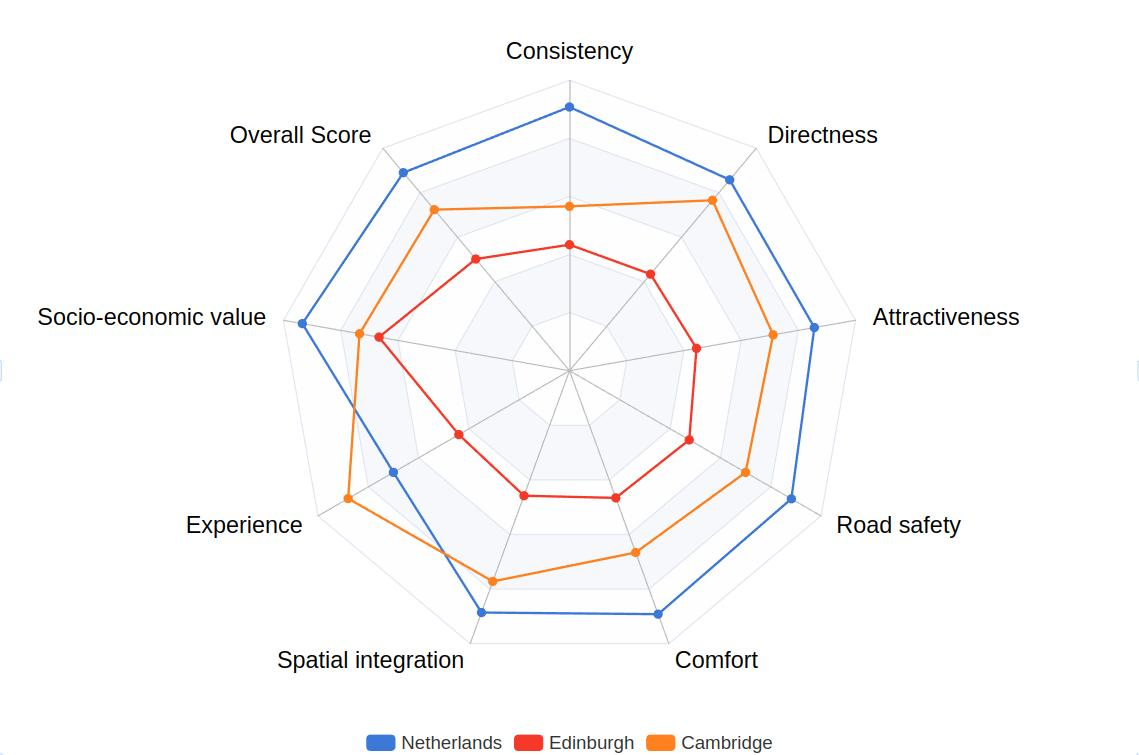
\includegraphics{figures/bicycle_infrastructure_scores.jpg}
    \caption{Spider web diagram comparing the Bicycle Infrastructure Scores (\cite{hull_bicycle_2014}).}
    \label{fig:bicycleinfrastructurescores}
\end{figure}

\subsection{Weather Conditions}
\label{litrev:weatherconditions}
Weather conditions will also have a pivotal effect on how a route planner will calculate the safest route for a cyclist. Following on from Cycling Infrastructure \see{litrev:cyclinginfrastructure}, it is demonstrated how a lack of good infrastructure goes hand-in-hand with creating an unsafe route alongside the weather. To ensure the safety of cyclists, all routes and road surfaces must be maintained to withstand different weather conditions (\cite{shoman_evaluation_2023}).

The weather also impacts a cyclist's likelihood to ride; Flynn states that cyclists `were nearly twice as likely to commute by bicycle when there was no morning precipitation' (\cite{flynn_weather_2012}). Even minor changes in the weather can drastically affect a cyclist's decision to ride, further demonstrating how vital the perceived safety of cycling is in deciding whether to ride. 

Contrasting this, Hull and O'Holleran state that the main environmental barriers included too much traffic, too many hills, no bike lanes/trails, no safe place to cycle and badly maintained streets (\cite{hull_bicycle_2014}). Therefore suggests that the weather should have a minimal impact on a cyclist's decision to ride if the infrastructure is sufficient. Despite the findings of Hull and O'Holleran, it seems to be a common finding that the perceived safety of cycling, both concerning the changing weather conditions and cycling infrastructure, is the primary factor in choosing cycling over an alternative method of transport. Miranda-Moreno and Nosal have shown how when infrastructure is implemented, there is generally an increase in total bicycle usage and diversion of cyclist flows away from roads to purpose-built infrastructure even in less ideal weather conditions (\cite{miranda-moreno_weather_2011}).

\section{Conclusion}
\label{litrev:conclusion}

To conclude, route planning with different customisable preferences has been implemented by a range of different existing organisations; however, focusing on a risk-based routing approach has not been addressed by these existing solutions. Utilising pre-existing routing algorithms such as OpenRouteService (\cite{noauthor_openrouteservice_nodate}) or Open Source Routing Machine (\cite{noauthor_project_nodate}) and integrating custom, weather and infrastructure data alongside the usual user-preferences has not been implemented within existing solutions. Therefore, this enables a unique system to be developed whereby crowd-sourced infrastructure data alongside weather data provided by OpenWeatherMap combined form a risk index utilised in a customised routing algorithm.
